Four elementary interactions are responsible for all the physical phenomena observed in the universe, each manifested by a force called fundamental force. Those are strong nuclear interaction, electromagnetic interaction, weak interaction and gravitational interaction. In classical physics, the laws of gravitation and electromagnetism were considered as axioms. However with regard to fields, these theoretical forces are worked out by the exchange of virtual bosons. The standard model of particle physics describes electromagnetic interactions, weak\cite{osti_4767615,PhysRevLett.19.1264}, and strong interactions. However, for arbitrary high energies, a quantum field theory has not yet been able to develop for gravity. 

The interpretation of gravity buries a handful of mysteries due to its different classical formulation. Einstein's principal of equivalence which couples matter to the stress tensor, and quantum mechanics which requires a positive energy implies that gravity is always attractive. Such a characteristic makes the theory of gravity singular at a certain point\cite{PhysRevD.14.2460}. At the singularity the classical description of gravity as well as the rest of the known laws of physics break down and a theory of quantum gravity is necessary to have a complete description of earliest stages of the universe where quantum effects are dominant.

In the pursue of a quantum theory of gravity, it is preferable to contemplate easy systems. Black holes offer, as toy models, a window to study quantum gravity, and are therefore at the forefront of current research. These mysterious objects are gravitational solutions to Einstein equations\cite{Schwarzschild:1916uq} with very special properties, some of them not well understood. In the 70's, Hawking discovered \cite{Hawking1975} that when coupled with quantum field theory, black holes have a temperature
\begin{equation}\label{Hawking temperature}
    T = \frac{\hbar \kappa}{2\pi},
\end{equation}
with $\kappa$ the surface gravity. These objects also come with an entropy proportional to their horizon area as brought to light by Bekenstein\cite{Bekenstein1972},
\begin{equation}\label{beken}
    S_{\text{gen}} = \frac{\text{Area}}{4\hbar G_N} + S_{outside}.
\end{equation}

These results show that black holes are objects with large, but finite, degrees of freedom, obeying ordinary laws of physics. Following these results, Almheiri and friends \cite{almheiri2020entropy} put a hypothesis called the "central dogma",
\begin{quote}
    As seen from the outside, a black hole can be described in terms of a quantum system with Area$/\left(4G_\text{N}\right)$ degrees of freedom, which evolves unitarily under time evolution.
\end{quote}

Even though it is an assumption, there is a lot of evidence coming from computations in super-symmetric string theories and matrix models that compute scattering amplitudes in special vacua\cite{Strominger_1996}. Another supporting evidence comes from the AdS/CFT correspondence. In holographic theories, a black hole and its surrounding environment is equivalently described by a conformal field theory living in the boundary of spacetime.

\begin{figure}
    \centering
     \begin{subfigure}[b]{0.3\textwidth}
        \centering
        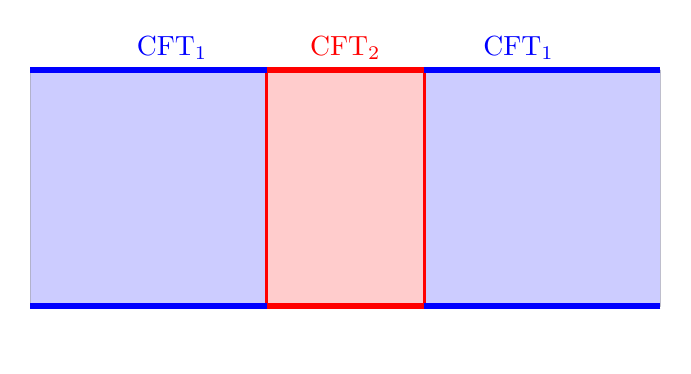
\begin{tikzpicture}
            \draw[fill=blue,opacity=0.2] (-4,3) -- (-1,3) -- (-1,0) -- (-4,0) -- (-4,3);
            \draw[fill=blue,opacity=0.2] (4,3) -- (1,3) -- (1,0) -- (4,0) -- (4,3);
            \draw[fill=red,opacity=0.2] (-1,3) -- (-1,0) -- (1,0) -- (1,3) -- (-1,3);
            \draw[red, line width=2] (-1,3) -- (1,3);
            \draw[red, line width=1] (-1,3) -- (-1,0);
            \draw[red, line width=1] (1,3) -- (1,0);
            \draw[red, line width=2] (-1,0) -- (1,0);
            \draw[blue, line width=2] (-4,3) -- (-1,3);
            \draw[blue, line width=2] (4,3) -- (1,3);
            \draw[blue, line width=2] (-4,0) -- (-1,0);
            \draw[blue, line width=2] (4,0) -- (1,0);
            \filldraw[red] (0,3) circle (0pt) node[anchor=south]{CFT$_2$};
            \filldraw[blue] (-2.2,3) circle (0pt) node[anchor=south]{CFT$_1$};
            \filldraw[blue] (2.2,3) circle (0pt) node[anchor=south]{CFT$_1$};
            \draw[opacity=0] (0,-.5) -- (0,0);
        \end{tikzpicture}
        \caption{}
        \label{itro 1}
     \end{subfigure}
     \hfill
     \begin{subfigure}[b]{0.3\textwidth}
        \centering
        \begin{tikzpicture}
        \draw[name path = A] (1.82,-.829) arc (335.5:440.5:2);
        \draw[name path = AA] (1.82,-.829) arc (335.5:80:2);
            \begin{scope}
                \draw  [clip] (0,0) circle (2cm);
                \draw[color=red,line width=.6mm, name path = B] (1.82,-.829) .. controls (.51,.51) .. (0.32,1.974);
                \draw[color=blue,line width=.5mm, name path = R] (1.80,-.872) .. controls (.47,.47) .. (0.28,1.98);
                \tikzfillbetween[of=A and B]{red, opacity=0.2};
                \tikzfillbetween[of=AA and R]{blue, opacity=0.2};
            \end{scope}
            \draw[red] node at (2,1){~~~~CFT$_2$};
            \draw[blue] node at (-2,-1){CFT$_1$~~~~};
         \end{tikzpicture}
        \caption{}
        \label{intro 2}
     \end{subfigure}
    \caption{(a) Two CFTs separated with a static interface. Time flows upwards. (b) The holographic dual of the two CFTs featuring a domain wall in the bulk separating the two geometries.}
    \label{the intro system}
\end{figure}

All of these important discoveries show that black holes are thermal objects and therefore are not completely black after all. With a temperature different than 0, black holes radiate and evaporate through time as shown by Hawking \cite{Hawking1975}. The essential question behind the evaporation is whether this process can be described under a unitary evolution. According to Hawking's calculations, the thermal entropy of radiations is an increasing function of time, starting at 0 when no Hawking quanta is radiated yet. As the black hole evaporates, the newly emitted radiations grow the entropy until the final stage where the entropy reaches a certain saturation and remains constant.

The increase of the entropy at early stages is expected until it reaches a value equal to one quarter of the area of the horizon. This quantity (\ref{beken}) represents the thermodynamic entropy of the black hole. Surpassing this value would mean that black holes somehow produce information greater than what they store. According to D. Page\cite{PhysRevLett.71.3743}, the von Neumann entropy should start decreasing once it reaches this point, called the Page time, until it reaches 0 at the end of the evaporation process. This decrease of entropy was later understood by means of QES (Quantum Extremal Surface). The von Neumann entropy formula goes as follow\cite{almheiri2020entropy},
\begin{equation}
    S = \text{min}_X\left\{\text{ext}_X\left[\frac{\text{Area}\left(X\right)}{4\hbar G_N} + S_\text{semi-cl}\left(\Sigma_X\right)\right]\right\},
\end{equation}
where $X$ is the QES which we minimize over. Computations result in two extremal surfaces one of which features an island behind the horizon belonging to the radiation slice. This island grows in the heart of the black hole eating up the inside, resulting in an overall decrease of the entanglement entropy.

In this note, we will consider a gravitational system featuring a thin static domain wall separating two geometries as represented in figure \ref{the intro system}. The left and right side of the domain wall are parts of different gravitational solutions: thermal AdS or BTZ black hole. The dual setup consists of two CFTs separated by an interface. This system has been studied in several recent papers\cite{Simidzija_2020, Bachas_2002, DeWolfe_2002}. We follow in this note mainly the analysis presented in \cite{Bachas_2021}. The Einstein-Hilbert action of our toy model is
\begin{equation}\label{action cft}
    \begin{split}
        I = -\frac{1}{2}\int_{\mathbb{S}_1}\text{d}^3x\sqrt{g_1}(R_1&+\frac{2}{\ell_1^2}) -\frac{1}{2}\int_{\mathbb{S}_2}\text{d}^3x\sqrt{g_2}(R_2+\frac{2}{\ell_2^2})\\
        & +\lambda  \int_{\mathbb{W}} \text{d}^2s\sqrt{\hat{g}_\omega} + \text{GHY} + \text{ct.}
    \end{split}
\end{equation}
where $S_i$ is the $i^\text{th}$ slice of the bulk geometry, $g_i$, $R_i$ and $l_i$ respectively its corresponding metric Ricci scalar and AdS radius. The domain wall with an induced metric $\hat{g}$ is described by its tension $\lambda$. The GHY term and the counter-term is computed in \cite{Bachas_2021}.

In particular we are interested in a situation where one slice has a very large number of degrees of freedom compared to the other slice which has a larger border. Following \cite{almheiri2019islands,Almheiri_2020}, we consider our gravitational system to be a finite portion containing the whole slice with the largest central charge. This setup can be described in three alternatives as can be seen in figure \ref{QM fig} where our system of interest is highlighted in yellow.

\begin{figure}
     \centering
     \begin{subfigure}[b]{0.3\textwidth}
        \centering
        \begin{tikzpicture}
            \draw (-2.5,3) -- (2.5,3);
            \draw[yellow, line width=2] (-1.3,3) -- (1.3,3);
            \filldraw[red] (-1,3) circle (2pt) node[anchor=south]{};
            \filldraw[red] (1,3) circle (2pt) node[anchor=south]{};
            \filldraw[red] (0,3) circle (0pt) node[anchor=south]{CFT$_2$};
            \filldraw[blue] (-1.9,3) circle (0pt) node[anchor=south]{CFT$_1$};
            \filldraw[blue] (1.9,3) circle (0pt) node[anchor=south]{CFT$_1$};
            \draw[opacity=0] (0,0) -- (0,3);
        \end{tikzpicture}
        \caption{}
        \label{QM 1}
     \end{subfigure}
     \hfill
     \begin{subfigure}[b]{0.3\textwidth}
         \centering
         \begin{tikzpicture}
            \draw (-2.5,3) -- (2.5,3);
            \draw[name path = x] (-2.5,3) -- (-1,3);
            \draw[name path = xx] (2.5,3) -- (1,3);
            \draw[name path = xxx] (-1,3) -- (1,3);
            \draw[opacity=0, name path = y] (-2.5,3) -- (-2.5,0) -- (-1,0) .. controls (-.6,1) and (-1.4,2) .. (-1,3);
            \draw[opacity=0, name path = yy] (2.5,3) -- (2.5,0) -- (1,0) .. controls (.6,1) and (1.4,2) .. (1,3);
            \draw[opacity=0, name path = yyy] (-1,3) .. controls (-1.4,2) and (-.6,1) .. (-1,0) -- (1,0) .. controls (.6,1) and (1.4,2) .. (1,3);
            \tikzfillbetween[of= y and x]{blue, opacity=0.2};
            \tikzfillbetween[of= yy and xx]{blue, opacity=0.2};
            \tikzfillbetween[of= yyy and xxx]{red, opacity=0.2};
            \draw[yellow, line width=2] (-1.3,3) -- (1.3,3);
            \filldraw[red] (-1,3) circle (2pt) node[anchor=south]{};
            \filldraw[red] (1,3) circle (2pt) node[anchor=south]{};
            \draw[color=red] (-1,3) .. controls (-1.4,2) and (-.6,1) .. (-1,0);
            \draw[color=red] (1,3) .. controls (1.4,2) and (.6,1) .. (1,0);
            \filldraw[red] (0,3) circle (0pt) node[anchor=south]{CFT$_2$};
            \filldraw[blue] (-1.9,3) circle (0pt) node[anchor=south]{CFT$_1$};
            \filldraw[blue] (1.9,3) circle (0pt) node[anchor=south]{CFT$_1$};
    \end{tikzpicture}
         \caption{}
         \label{QM 2}
     \end{subfigure}
     \hfill
     \begin{subfigure}[b]{0.3\textwidth}
         \centering
         \begin{tikzpicture}
            \draw (0,3) -- (4,3);
            \filldraw[yellow] (0,3) circle (5pt) node[anchor=south]{QM};
            \draw[yellow, line width=2] (0,3) -- (1,3);
            \draw (1,2.8) -- (1,3.2);
            \draw (.9,2.8) -- (1,2.8);
            \draw (.9,3.2) -- (1,3.2);
            \draw[opacity=0] (0,0) -- (0,3);
            \filldraw[blue] (3,3) circle (0pt) node[anchor=south]{CFT$_1$};
        \end{tikzpicture}
         \caption{}
         \label{QM 3}
     \end{subfigure}
     \hfill
    \caption{(a) CFT$_1$  and CFT$_2$ respectively with central charges $c_1\ll c_2$ and boundaries $L_1\gg L_2$. These are separated by an interface shown in red circles. (b) The holographic dual of the two CFTs featuring a domain wall with tension $\lambda$ separating between the two geometries. (c) Our gravitational system with large degrees of freedom represented by a quantum dot following the central dogma, with a small slice of the bath region.}
    \label{QM fig}
\end{figure}

The goal of this study is to study the behaviour of the entanglement entropy of the yellow region. This will require purifying the thermal state by virtue of the thermofield double state, dual to the double sided  geometry\cite{ISRAEL1976107}. The computation of  RT surfaces will follow. We expect a rising entropy as a function of time, and a saturating constant entropy at late times.

This note is organised as follows. In chapter \ref{section 2} we present a review of entanglement entropy in the frame work of quantum mechanics as well as field theory. In chapter \ref{section 3}, we review the holographic computation of entanglement entropy proposed by S. Ryu and T. Takayanagi\cite{Ryu, Ryu_2006} with explicit calculations for two examples: vacuum CFT and BTZ black hole. In chapter \ref{section 4} we present briefly the thermodynamic equations behind black hole dynamics. We summarise Hawking information paradox as well as its solution by means of QES. In chapter \ref{section 5} we review the work presented in \cite{Bachas_2021} regarding Holographic ICFTs. We then consider the limit of interest with a large bath $L_1\gg L_2$ and large degrees of freedom in the other side $c_1\ll c_2$. We find the dominant phase and pursue its study in the next chapter \ref{section 6}. We compute the RT surfaces through geodesic calculations. In chapter \ref{section 7} we give the double sided geometry of the dominant phase, dual to a pure CFT state living on its double boundary. We then compute RT surfaces in the double sided geometry. We find that the entropy of our system follows a Page curve. 
